\documentclass[12pt,a4paper]{article}

% 中文支持
\usepackage{ctex}

% 页面设置
\usepackage{geometry}
\geometry{left=2.5cm,right=2.5cm,top=2.5cm,bottom=2.5cm}

% 颜色
\usepackage{xcolor}
\definecolor{marioblue}{RGB}{92,148,252}
\definecolor{mariored}{RGB}{231,0,18}
\definecolor{mariogreen}{RGB}{0,170,0}
\definecolor{marioyellow}{RGB}{255,215,0}

% 图形
\usepackage{tikz}
\usetikzlibrary{shapes,arrows,positioning,calc}

% 列表
\usepackage{enumitem}
\setlist[itemize]{leftmargin=2em}

% 标题样式
\usepackage{titlesec}
\titleformat{\section}{\Large\bfseries\color{mariored}}{\thesection}{1em}{}
\titleformat{\subsection}{\large\bfseries\color{marioblue}}{\thesubsection}{1em}{}

% 页眉页脚
\usepackage{fancyhdr}
\pagestyle{fancy}
\fancyhf{}
\fancyhead[L]{\small 齐秦快跑}
\fancyhead[R]{\small 游戏说明书}
\fancyfoot[C]{\thepage}
\renewcommand{\headrulewidth}{0.5pt}

% 超链接
\usepackage{hyperref}
\hypersetup{colorlinks=true,linkcolor=marioblue,urlcolor=mariored}

% 盒子
\usepackage{tcolorbox}
\tcbuselibrary{skins,breakable}

\newtcolorbox{gamebox}[1][]{
  colback=white,
  colframe=marioblue,
  fonttitle=\bfseries,
  title=#1,
  arc=3mm,
  boxrule=2pt,
  left=5pt,right=5pt,top=5pt,bottom=5pt
}

\newtcolorbox{tipbox}{
  colback=marioyellow!20,
  colframe=marioyellow!80!black,
  arc=2mm,
  boxrule=1pt,
  left=5pt,right=5pt,top=5pt,bottom=5pt
}

\begin{document}

% 封面
\begin{titlepage}
\begin{tikzpicture}[remember picture,overlay]
  % 背景
  \fill[marioblue] (current page.south west) rectangle (current page.north east);
  
  % 云朵装饰
  \foreach \x/\y in {2/20,8/18,14/22,18/16} {
    \fill[white] (\x,\y) circle (0.8);
    \fill[white] (\x+0.6,\y+0.3) circle (0.6);
    \fill[white] (\x-0.6,\y+0.2) circle (0.5);
  }
  
  % 地面
  \fill[mariogreen] (0,0) rectangle (22,3);
  \draw[line width=3pt] (0,3) -- (22,3);
\end{tikzpicture}

\vspace*{8cm}

\begin{center}
  {\fontsize{60}{72}\selectfont\bfseries\color{white}
  \textcolor{mariored}{齐}\textcolor{marioyellow}{秦}\textcolor{mariored}{快}\textcolor{marioyellow}{跑}}
  
  \vspace{1cm}
  
  {\Large\color{white} 游戏使用说明书}
  
  \vspace{3cm}
  
  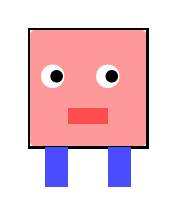
\begin{tikzpicture}
    % 主角齐秦
    \fill[pink!80!red,rounded corners=3pt] (0,0) rectangle (1.5,1.5);
    \draw[line width=1pt] (0,0) rectangle (1.5,1.5);
    % 眼睛
    \fill[white] (0.3,0.9) circle (0.15);
    \fill[black] (0.35,0.9) circle (0.08);
    \fill[white] (1.0,0.9) circle (0.15);
    \fill[black] (1.05,0.9) circle (0.08);
    % 嘴巴
    \fill[red!70] (0.5,0.3) rectangle (1.0,0.5);
    % 腿
    \fill[blue!70] (0.2,-0.5) rectangle (0.5,0);
    \fill[blue!70] (1.0,-0.5) rectangle (1.3,0);
  \end{tikzpicture}
  
  \vspace{2cm}
  
  {\large\color{white} 版本 1.0}
  
  \vspace{0.5cm}
  
  {\large\color{white} \today}
\end{center}
\end{titlepage}

% 目录
\tableofcontents
\newpage

% 第一章：游戏简介
\section{游戏简介}

\begin{gamebox}[游戏概述]
《齐秦快跑》是一款灵感来源于经典游戏《超级马里奥》的横版跑酷游戏。玩家将控制主角"齐秦"在充满挑战的赛道上奔跑，躲避各种障碍物，收集道具，尽可能跑得更远、获得更高分数。
\end{gamebox}

\subsection{游戏背景}

齐秦是一个热爱运动的小伙伴，他喜欢在蓝天白云下奔跑。但是，路上充满了各种障碍物：网球网会让他掉血掉牙，糖果会让他噎住，还有球会让他晕倒。幸运的是，他的朋友王九骁会在路上帮助他回血！

\subsection{游戏特色}

\begin{itemize}
  \item \textbf{马里奥风格画面}：经典的蓝色天空、绿色草地、像素风格的人物设计
  \item \textbf{简单易上手}：只需按空格键即可控制跳跃
  \item \textbf{丰富的障碍物}：网球网、糖果、球、王九骁等多种元素
  \item \textbf{BUFF系统}：噎住掉血、眩晕停顿、回血等多种状态效果
  \item \textbf{背景音乐}：游戏时自动播放背景音乐
\end{itemize}

% 第二章：操作说明
\section{操作说明}

\subsection{基本操作}

\begin{center}
\begin{tikzpicture}[node distance=2cm]
  \node[draw,fill=marioyellow!30,rounded corners,minimum width=4cm,minimum height=1cm] (key) {\Large\bfseries 空格键 (Space)};
  \node[right of=key,node distance=5cm,align=left] {跳跃};
  \draw[->,line width=2pt,mariored] (key) -- ++(3,0);
\end{tikzpicture}
\end{center}

\begin{tipbox}
\textbf{提示}：齐秦会自动向前奔跑，玩家只需要控制跳跃时机来躲避障碍物即可！
\end{tipbox}

\subsection{游戏界面}

游戏界面包含以下元素：

\begin{enumerate}
  \item \textbf{左上角}：血量条和牙齿数量显示
  \item \textbf{右上角}：当前分数和奔跑距离
  \item \textbf{中央}：主角齐秦
  \item \textbf{背景}：马里奥风格的蓝天白云和绿色草地
\end{enumerate}

% 第三章：游戏元素
\section{游戏元素}

\subsection{主角：齐秦}

\begin{center}
\begin{tikzpicture}[scale=1.5]
  % 身体
  \fill[pink!80!red,rounded corners=3pt] (0,0) rectangle (1.5,1.5);
  \draw[line width=1pt] (0,0) rectangle (1.5,1.5);
  % 眼睛
  \fill[white] (0.3,0.9) circle (0.15);
  \fill[black] (0.35,0.9) circle (0.08);
  \fill[white] (1.0,0.9) circle (0.15);
  \fill[black] (1.05,0.9) circle (0.08);
  % 嘴巴
  \fill[red!70] (0.5,0.3) rectangle (1.0,0.5);
  % 腿
  \fill[blue!70] (0.2,-0.5) rectangle (0.5,0);
  \fill[blue!70] (1.0,-0.5) rectangle (1.3,0);
  
  % 标注
  \draw[->,line width=1pt] (2,1.2) -- (1.6,0.9) node[midway,above right] {\small 齐秦};
\end{tikzpicture}
\end{center}

齐秦是游戏的主角，一个粉色方块小人，有8颗牙齿。当受到伤害时会掉牙，牙齿掉光或血量为0时游戏结束。

\subsection{障碍物与道具}

\begin{gamebox}[网球网]
\begin{center}
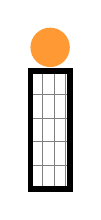
\begin{tikzpicture}[scale=1]
  % 网
  \foreach \y in {0,0.3,...,1.5} {
    \draw[gray] (0,\y) -- (0.5,\y);
  }
  \foreach \x in {0,0.15,...,0.5} {
    \draw[gray] (\x,0) -- (\x,1.5);
  }
  \draw[line width=2pt] (0,0) rectangle (0.5,1.5);
  % 顶部的球
  \fill[orange!80] (0.25,1.8) circle (0.25);
\end{tikzpicture}
\end{center}

\textbf{效果}：掉血 + 掉牙

碰到网球网会损失血量，并且会掉一颗牙齿。连续碰到会快速掉血掉牙，非常危险！
\end{gamebox}

\vspace{0.5cm}

\begin{gamebox}[糖果 🍬]
\begin{center}
{\Large 🍬}
\end{center}

\textbf{效果}：噎住卡顿 + 持续掉血

碰到糖果会噎住2秒钟，期间会持续掉血（每0.2秒掉1点血）。只有碰到王九骁才能停止掉血！
\end{gamebox}

\vspace{0.5cm}

\begin{gamebox}[球 ⚽]
\begin{center}
{\Large ⚽}
\end{center}

\textbf{效果}：晕倒停顿1.5秒

碰到球会晕倒，屏幕出现星星，无法操作1.5秒。期间可能碰到其他障碍物！
\end{gamebox}

\vspace{0.5cm}

\begin{gamebox}[王九骁]
\begin{center}
\begin{tikzpicture}[scale=1.2]
  % 身体
  \fill[mariogreen,rounded corners=2pt] (0,0) rectangle (1,1);
  \draw[line width=1pt] (0,0) rectangle (1,1);
  % 眼睛
  \fill[white] (0.2,0.6) circle (0.12);
  \fill[black] (0.25,0.6) circle (0.06);
  \fill[white] (0.65,0.6) circle (0.12);
  \fill[black] (0.7,0.6) circle (0.06);
  % 嘴巴
  \fill[red!60] (0.35,0.2) rectangle (0.65,0.35);
  % 腿
  \fill[blue!70] (0.1,-0.4) rectangle (0.35,0);
  \fill[blue!70] (0.65,-0.4) rectangle (0.9,0);
  % 名字
  \node[above] at (0.5,1.1) {\tiny\bfseries 王九骁};
\end{tikzpicture}
\end{center}

\textbf{效果}：回血30点 + 停止噎住掉血

王九骁是齐秦的好朋友！碰到他可以回血30点，如果正在噎住掉血，也会立即停止。王九骁的移动速度是齐秦的一半。
\end{gamebox}

% 第四章：游戏规则
\section{游戏规则}

\subsection{胜利条件}

游戏没有终点，目标是：
\begin{itemize}
  \item 尽可能跑得更远
  \item 获得更高的分数
  \item 保持血量健康
  \item 保留更多的牙齿
\end{itemize}

\subsection{失败条件}

满足以下任一条件时游戏结束：

\begin{enumerate}
  \item \textbf{血量为0}：受到太多伤害
  \item \textbf{牙齿掉光}：8颗牙齿全部掉落
\end{enumerate}

\begin{tipbox}
\textbf{重要提示}：牙齿掉光也会游戏结束！所以不仅要关注血量，还要注意保护牙齿。
\end{tipbox}

\subsection{计分规则}

\begin{itemize}
  \item 奔跑距离 $\times$ 10 = 当前分数
  \item 游戏速度会逐渐加快
  \item 跑得越远，难度越高
\end{itemize}

% 第五章：游戏技巧
\section{游戏技巧}

\subsection{基础技巧}

\begin{enumerate}
  \item \textbf{节奏跳跃}：掌握好跳跃的节奏，不要过早或过晚
  \item \textbf{连续障碍}：注意多个障碍物连续出现的情况
  \item \textbf{优先躲避}：网球网最危险，优先躲避
\end{enumerate}

\subsection{进阶技巧}

\begin{enumerate}
  \item \textbf{主动找王九骁}：如果噎住了，主动寻找王九骁回血
  \item \textbf{预判位置}：观察障碍物出现规律，提前预判
  \item \textbf{保持冷静}：晕倒时不要慌张，醒来后迅速调整
\end{enumerate}

% 第六章：技术信息
\section{技术信息}

\subsection{系统要求}

\begin{itemize}
  \item 现代浏览器（Chrome、Firefox、Safari、Edge等）
  \item 支持HTML5和JavaScript
  \item 建议分辨率：1280x720或更高
\end{itemize}

\subsection{游戏文件}

\begin{itemize}
  \item \texttt{index.html}：游戏主文件
  \item \texttt{back.mp3}：背景音乐
  \item \texttt{copy.png}：启动画面图片
\end{itemize}

\subsection{开源技术}

本游戏使用以下开源技术：
\begin{itemize}
  \item GSAP (GreenSock Animation Platform) - 动画库
  \item HTML5 Canvas - 游戏渲染
\end{itemize}

% 结语
\section*{结语}

\begin{center}
\begin{tikzpicture}
  \node[draw=mariored,line width=2pt,rounded corners=10pt,inner sep=15pt,fill=white] {
    \begin{minipage}{0.7\textwidth}
    \centering
    \Large\bfseries
    祝你在《齐秦快跑》中\\[0.5em]
    跑得更远，跳得更高！
    \end{minipage}
  };
\end{tikzpicture}
\end{center}

\vspace{1cm}

\begin{center}
\textit{游戏版本 1.7 | 最后更新：\today}
\end{center}

\end{document}
